% !TEX encoding = UTF-8 Unicode
\documentclass[11pt,a4paper]{report}
\usepackage[french]{babel}
\usepackage[T1]{fontenc}
\usepackage[utf8]{inputenc}
\usepackage{microtype}
\usepackage{geometry}
\geometry{margin=2.5cm}
\usepackage{graphicx}
\usepackage{booktabs}
\usepackage{hyperref}
\usepackage{xcolor}
\hypersetup{colorlinks=true,linkcolor=blue!60!black,urlcolor=blue!60!black}

\title{Rapport REESO\\[0.6em]
\large Analyse des déplacements forcés de population — Burkina Faso\\
\large TP-02 — Projet final FADP/REESO 2026}
\author{Bassana — Formation Analyse de données avec Python (REESO)}
\date{Remise : 10 avril 2026}

% ---------------------------------------------------------------------------
% Constantes numériques — alignées sur le notebook
% « TP integration Theme 2.ipynb » (même pipeline : df_geo, extract_region, etc.)
% Mettre à jour ce fichier après ré-exécution complète du notebook si les données changent.
%
% Vérification rapide : rejouer les cellules du notebook et reporter ici les valeurs
% affichées pour resume_region, corrélations, prévision, etc.
% ---------------------------------------------------------------------------
\newcommand{\EventsGeo}{25}
\newcommand{\TotalDeplaces}{61\,746}
\newcommand{\MedianeEvt}{1\,536}
\newcommand{\PcentVingtCinq}{2\,868}
\newcommand{\PcentQuatreVingtDix}{3923{,}4}
\newcommand{\NbMassifs}{3}
\newcommand{\NbHotspots}{2}
\newcommand{\DailyMax}{18\,682}
\newcommand{\CroissanceMoyPct}{36{,}92}
\newcommand{\CorrDist}{0{,}402}
\newcommand{\Rdeux}{0{,}147}
\newcommand{\PrevisionMois}{6\,324}
\newcommand{\DateMin}{2025-09-16}
\newcommand{\DateMax}{2026-02-13}
\newcommand{\MoisMax}{2025-11}
\newcommand{\MoisMaxVal}{18\,682}
\newcommand{\EcartType}{2\,290{,}6}
\newcommand{\CoeffVar}{92{,}7}

% Agrégations par région (groupby region sur df_geo)
\newcommand{\RegBdmEvts}{10}
\newcommand{\RegBdmTotal}{36\,783}
\newcommand{\RegBdmMoy}{3\,678{,}3}
\newcommand{\RegNordEvts}{9}
\newcommand{\RegNordTotal}{17\,695}
\newcommand{\RegNordMoy}{1\,966{,}1}
\newcommand{\RegEstEvts}{5}
\newcommand{\RegEstTotal}{5\,898}
\newcommand{\RegEstMoy}{1\,179{,}6}
\newcommand{\RegCNordEvts}{1}
\newcommand{\RegCNordTotal}{1\,370}
\newcommand{\RegCNordMoy}{1\,370{,}0}


\begin{document}

\maketitle

\begin{abstract}
\noindent
Ce rapport synthétise l'analyse réalisée dans le notebook \texttt{TP integration Theme 2.ipynb}
sur le jeu \texttt{event\_data\_bfa.csv} (IDMC). La structure suit les consignes du document
\textit{Projet final — FADP/REESO} : résumé, introduction, données et méthode, résultats,
discussion, recommandations et annexes. Les chiffres cités correspondent aux sorties du notebook
(pipeline \texttt{df\_geo}, agrégations et exports).
\end{abstract}

\tableofcontents
\clearpage

% --- Structure imposée (projet final) ---

\chapter{Résumé exécutif}

\paragraph{Contexte.}
Le Burkina Faso fait face à une crise humanitaire marquée par des déplacements internes de population.
Les données exploitées proviennent d'événements géolocalisés et datés dans \texttt{event\_data\_bfa.csv}.

\paragraph{Objectifs.}
Quantifier l'ampleur des déplacements, repérer les zones et périodes critiques, relier taille des
événements et distance à Ouagadougou, et proposer des pistes d'action pour les acteurs humanitaires.

\paragraph{Principaux résultats (notebook).}
Sur le périmètre géographiquement valide, on dénombre \EventsGeo{} événements totalisant
\TotalDeplaces{} personnes déplacées ; la médiane par événement est de \MedianeEvt{} personnes.
Les événements au-dessus du 90\textsuperscript{e} percentile (\PcentQuatreVingtDix{}) sont au
nombre de \NbMassifs{}. La corrélation linéaire entre distance à la capitale et \texttt{figure}
est $r = \CorrDist{}$. La tendance linéaire sur la série mensuelle des déplacés donne
$R^2 = \Rdeux{}$ et une projection « mois suivant » d'environ \PrevisionMois{} déplacés.

\paragraph{Recommandations clés.}
Prioriser les régions les plus touchées (Boucle du Mouhoun, Nord, Est), renforcer la veille sur les
périodes de pics, et harmoniser les libellés régionaux (Est/Nord, etc.) dans les chaînes
\texttt{locations\_name}.

\chapter{Introduction}

\section{Contexte du projet}
Travail individuel de clôture de la formation FADP/REESO : analyse complète d'un jeu réel
(\texttt{event\_data\_bfa.csv}) avec Python (pandas, numpy, matplotlib, seaborn), dans l'esprit
des consignes prévoyant un notebook structuré et un rapport PDF.

\section{Problématique}
Comprendre la répartition spatiale et temporelle des déplacements forcés et identifier où et quand
la réponse humanitaire doit être priorisée.

\section{Questions de recherche}
\begin{itemize}
  \item Q1 : Quelles régions et localités concentrent le plus de déplacés ?
  \item Q2 : Existe-t-il des pics temporels (mois, jours) ?
  \item Q3 : La distance à Ouagadougou est-elle liée à la taille des événements ?
  \item Q4 : Quels sont les « hotspots » au sens du notebook (somme $>1000$ et plus de 2 événements) ?
\end{itemize}

\section{Périmètre de l'étude}
\begin{itemize}
  \item Période couverte par les données : \DateMin{} à \DateMax{}.
  \item Après filtrage des coordonnées dans les bornes du Burkina (lat.\ 9--15, long.\ $-6$--3) :
  \EventsGeo{} événements retenus pour l'analyse spatiale (\texttt{df\_geo}).
  \item Variable principale : \texttt{figure} (nombre de personnes déplacées par événement).
\end{itemize}

\chapter{Données et méthodologie}

\section{Sources de données}
Fichier \texttt{event\_data\_bfa.csv} : coordonnées, dates de déplacement, effectifs \texttt{figure},
localisation textuelle (\texttt{locations\_name}).

\section{Description des variables (extrait notebook)}
Variables clés utilisées : \texttt{displacement\_date}, \texttt{figure}, \texttt{latitude},
\texttt{longitude}, \texttt{locations\_name}, \texttt{displacement\_start\_date},
\texttt{displacement\_end\_date} ; variables dérivées \texttt{mois}, \texttt{annee},
\texttt{duree\_jours}, \texttt{region}.

\section{Qualité des données}
Vérification des valeurs manquantes pour \texttt{latitude} / \texttt{longitude} ; exclusion des
lignes sans coordonnées ; contrôle des plages lat/long. Les types de déplacement dans la colonne
\texttt{category} sont en pratique peu renseignés sur cet extrait ; le notebook s'appuie surtout sur
\texttt{displacement\_type} et sur les agrégations géographiques.

\section{Nettoyage effectué}
\begin{itemize}
  \item Conversion des dates en \texttt{datetime} ; calcul de \texttt{duree\_jours}.
  \item Suppression des lignes sans coordonnées ; filtre géographique sur le Burkina.
  \item Extraction de la région depuis \texttt{locations\_name} (avant-dernier segment avant le pays),
  avec normalisation \texttt{East}$\rightarrow$\texttt{Est}, \texttt{North}$\rightarrow$\texttt{Nord},
  \texttt{Centre-Nord Region}$\rightarrow$\texttt{Centre-Nord}.
  \item Pour les chaînes avec plusieurs localités séparées par \texttt{;}, prise de la dernière localité
  pour l'extraction de la région (comme dans le notebook).
\end{itemize}

\section{Méthodes d'analyse}
\begin{itemize}
  \item Agrégations pandas : par mois, par région, par localité ; moyenne mobile 7 jours sur la série
  journalière.
  \item Statistiques numpy : médiane, percentiles, écart-type, coefficient de variation
  (\(\approx \CoeffVar{}\,\%\) ; écart-type \(\approx \EcartType{}\)).
  \item Distance à Ouagadougou (12{,}37 ; $-1{,}52$) : formule de haversine ; classes de distance
  \texttt{<50km}, \ldots\ puis corrélation avec \texttt{figure}.
  \item Tendance mensuelle : régression linéaire \texttt{np.polyfit} sur l'indice des mois ;
  prévision pour le mois suivant (même formule que dans le notebook).
  \item Visualisations : séries temporelles, barplots, heatmap, scatter géographique, figure 2$\times$2
  exportée en \texttt{rapport\_deplacements.png} (300 dpi).
\end{itemize}

\chapter{Résultats}

\section{Statistiques descriptives}
Effectif analysé : \EventsGeo{} événements totalisant \TotalDeplaces{} déplacés. Médiane \MedianeEvt{},
75\textsuperscript{e} percentile \PcentVingtCinq{}, 90\textsuperscript{e} percentile
\PcentQuatreVingtDix{}. Nombre d'événements « massifs » (strictement au-dessus du P90) : \NbMassifs{}.
Nombre de hotspots (critère notebook : somme $>1000$ et plus de 2 événements par localité) :
\NbHotspots{}.

\section{Analyses exploratoires}
\begin{itemize}
  \item Pic journalier de déplacés (somme \texttt{figure} par jour) : \DailyMax{}.
  \item Mois le plus chargé en somme mensuelle : \MoisMax{} (\MoisMaxVal{} déplacés au total sur le mois).
  \item Croissance moyenne mois à mois (sur les variations relatives de la série mensuelle) :
  environ \CroissanceMoyPct{}\,\% (à interpréter avec prudence sur une série courte).
\end{itemize}

\section{Tests / modélisation}
Pas de test d'hypothèse classique paramétrique dans le notebook ; indicateurs de liaison :
corrélation Pearson distance--effectif \CorrDist{} ; régression linéaire sur la série mensuelle avec
$R^2 = \Rdeux{}$ et projection \PrevisionMois{} déplacés pour le mois suivant (même calcul que la cellule
notebook « prévision »).

\section{Visualisations}
La figure principale synthétique est enregistrée sous \texttt{rapport\_deplacements.png} (générée par le
notebook).

\begin{figure}[htbp]
  \centering
  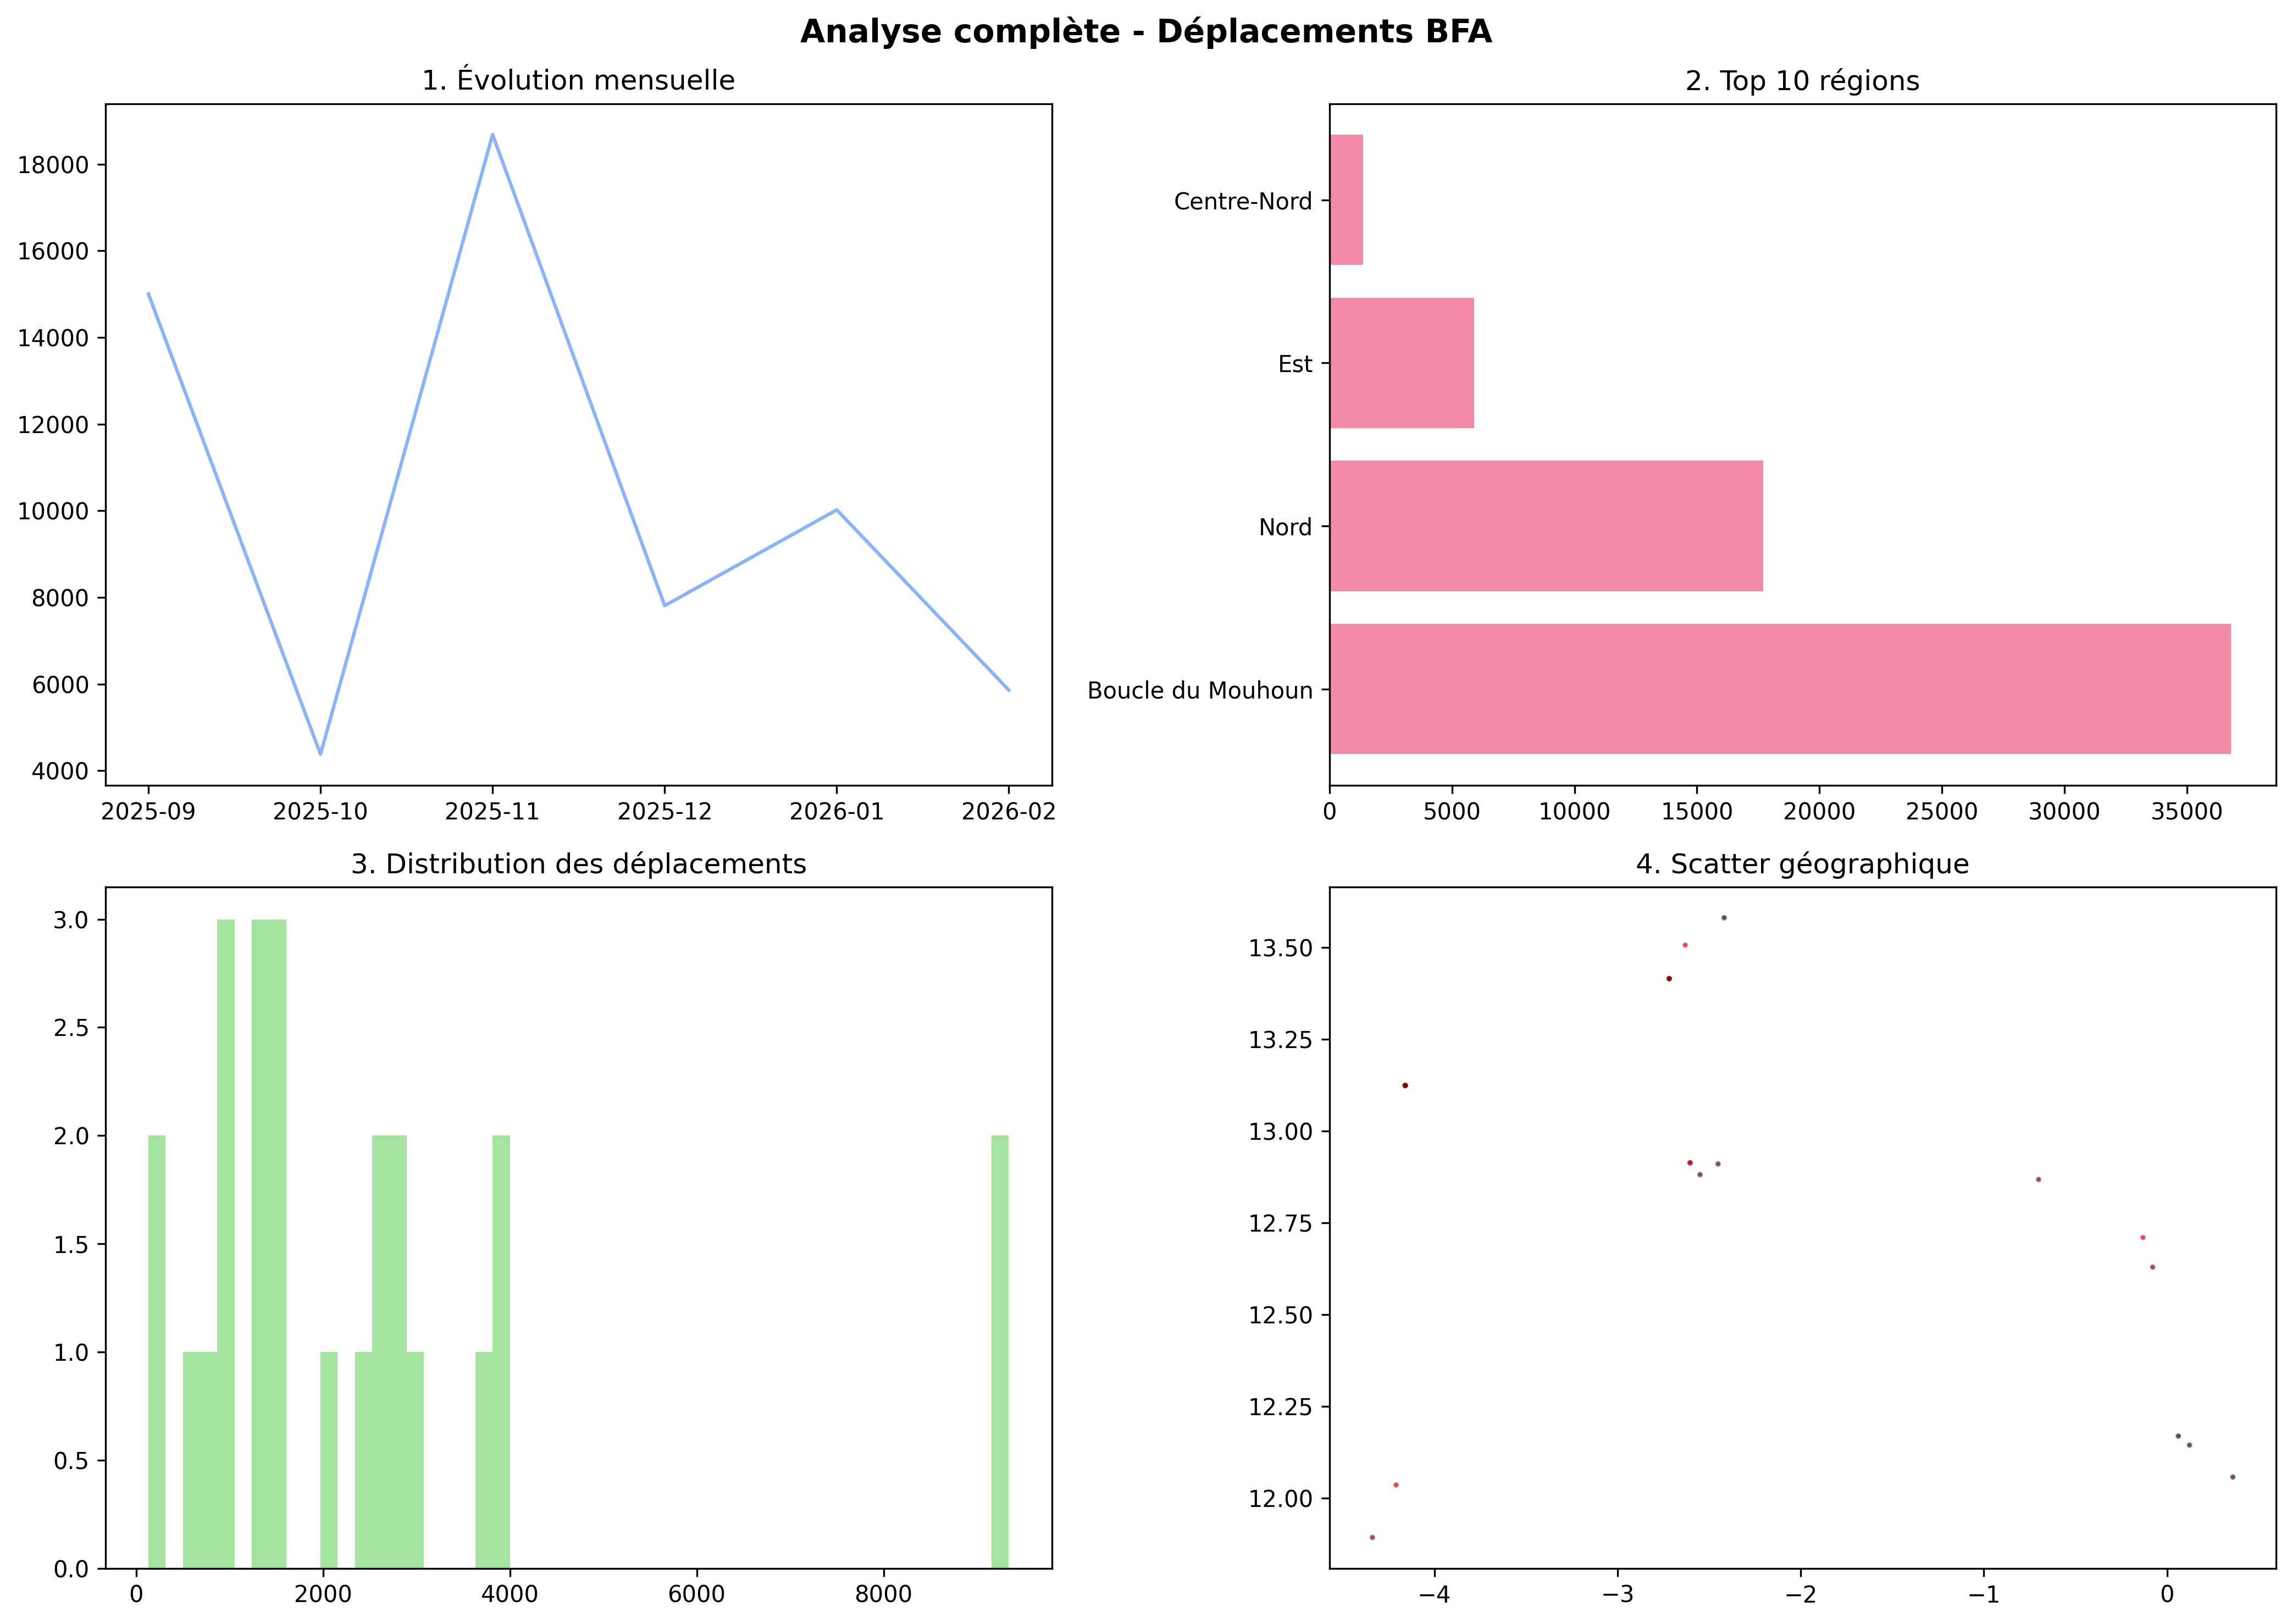
\includegraphics[width=\linewidth]{rapport_deplacements.png}
  \caption{Synthèse visuelle (export PNG 300 dpi) — notebook TP-02.}
\end{figure}

\section{Synthèse régionale}
\begin{table}[htbp]
  \centering
  \begin{tabular}{lrrr}
    \toprule
    Région & Événements & Total déplacés & Moy. / événement \\
    \midrule
    Boucle du Mouhoun & \RegBdmEvts & \RegBdmTotal & \RegBdmMoy \\
    Nord & \RegNordEvts & \RegNordTotal & \RegNordMoy \\
    Est & \RegEstEvts & \RegEstTotal & \RegEstMoy \\
    Centre-Nord & \RegCNordEvts & \RegCNordTotal & \RegCNordMoy \\
    \bottomrule
  \end{tabular}
  \caption{Agrégation par \texttt{region} (notebook, \texttt{df\_geo}).}
\end{table}

\chapter{Discussion}

\paragraph{Interprétation.}
La forte concentration sur la Boucle du Mouhoun et le Nord est cohérente avec la crise sécuritaire
décrite dans le contexte. La corrélation positive modérée avec la distance à Ouagadougou suggère que
les très gros volumes ne sont pas exclusivement périphériques.

\paragraph{Réponses aux questions.}
Q1--Q4 sont traitées quantitativement dans les sections précédentes ; les limites de
généralisation temporelle restent fortes (fenêtre courte, série mensuelle).

\paragraph{Limites.}
Échantillon réduit (\EventsGeo{} événements), une partie des champs catégoriels peu renseignés,
prévision linéaire très incertaine ($R^2$ faible).

\paragraph{Perspectives.}
Enrichir avec d'autres vagues, croiser des indicateurs sécuritaires ou climatiques, et documenter
les biais de géocodage.

\chapter{Recommandations}

\paragraph{Stratégiques.}
Mobiliser la réponse humanitaire en priorité sur les régions identifiées ; maintenir une cartographie
à jour des hotspots.

\paragraph{Plan d'action.}
Mettre en place des revues mensuelles des séries, valider les libellés géographiques en amont des
agrégations.

\paragraph{Indicateurs de suivi.}
Nombre mensuel de déplacés, nombre de hotspots, corrélation distance--effectif sur les nouvelles
fenêtres temporelles.

\chapter{Annexes}

\section*{Annexe A — Extrait de code (logique région)}
La fonction \texttt{extract\_region} du notebook utilise les alias Est/Nord et la dernière localité
lorsque \texttt{locations\_name} contient un point-virgule.

\section*{Annexe B — Fichiers produits par le notebook}
\texttt{Rapport\_Deplacements.xlsx}, \texttt{hotspots\_SIG.csv}, \texttt{rapport\_deplacements.md},
\texttt{rapport\_deplacements.png}.

\section*{Annexe C — Lien notebook}
À adapter : lien Google Colab (consigne projet) une fois le notebook publié en lecture seule.

\end{document}
